% ----------------------------------------------------
% Design
% ----------------------------------------------------
\documentclass[class=report,11pt,crop=false]{standalone}
% Page geometry
\usepackage[a4paper,margin=20mm,top=25mm,bottom=25mm]{geometry}

% Font choice
\usepackage{lmodern}

% Use IEEE bibliography style
\bibliographystyle{IEEEtran}

% Line spacing
\usepackage{setspace}
\setstretch{1.20}

% Ensure UTF8 encoding
\usepackage[utf8]{inputenc}

% Language standard (not too important)
\usepackage[english]{babel}

% Skip a line in between paragraphs
\usepackage{parskip}

% For the creation of dummy text
\usepackage{blindtext}

% Math
\usepackage{amsmath}

% Header & Footer stuff
\usepackage{fancyhdr}
\pagestyle{fancy}
\fancyhead{}
\fancyhead[R]{\nouppercase{\rightmark}}
\fancyfoot{}
\fancyfoot[C]{\thepage}
\renewcommand{\headrulewidth}{0.0pt}
\renewcommand{\footrulewidth}{0.0pt}
\setlength{\headheight}{13.6pt}

% Epigraphs
\usepackage{epigraph}
\setlength\epigraphrule{0pt}
\setlength{\epigraphwidth}{0.65\textwidth}

% Colour
\usepackage{color}
\usepackage[usenames,dvipsnames]{xcolor}

% Hyperlinks & References
\usepackage{hyperref}
\definecolor{linkColour}{RGB}{77,71,179}
\hypersetup{
    colorlinks=true,
    linkcolor=linkColour,
    filecolor=linkColour,
    urlcolor=linkColour,
    citecolor=linkColour,
}
\urlstyle{same}

% Automatically correct front-side quotes
\usepackage[autostyle=false, style=ukenglish]{csquotes}
\MakeOuterQuote{"}

% Graphics
\usepackage{graphicx}
\graphicspath{{Images/}{../Images/}}
\usepackage{makecell}
\usepackage{transparent}

% SI units
\usepackage{siunitx}

% Microtype goodness
\usepackage{microtype}

% Listings
\usepackage[T1]{fontenc}
\usepackage{listings}
\usepackage[scaled=0.8]{DejaVuSansMono}

% Custom colours for listings
\definecolor{backgroundColour}{RGB}{250,250,250}
\definecolor{commentColour}{RGB}{73, 175, 102}
\definecolor{identifierColour}{RGB}{196, 19, 66}
\definecolor{stringColour}{RGB}{252, 156, 30}
\definecolor{keywordColour}{RGB}{50, 38, 224}
\definecolor{lineNumbersColour}{RGB}{127,127,127}
\lstset{
  language=Matlab,
  captionpos=b,
  aboveskip=15pt,belowskip=10pt,
  backgroundcolor=\color{backgroundColour},
  basicstyle=\ttfamily,%\footnotesize,        % the size of the fonts that are used for the code
  breakatwhitespace=false,         % sets if automatic breaks should only happen at whitespace
  breaklines=true,                 % sets automatic line breaking
  postbreak=\mbox{\textcolor{red}{$\hookrightarrow$}\space},
  commentstyle=\color{commentColour},    % comment style
  identifierstyle=\color{identifierColour},
  stringstyle=\color{stringColour},
   keywordstyle=\color{keywordColour},       % keyword style
  %escapeinside={\%*}{*)},          % if you want to add LaTeX within your code
  extendedchars=true,              % lets you use non-ASCII characters; for 8-bits encodings only, does not work with UTF-8
  frame=single,	                   % adds a frame around the code
  keepspaces=true,                 % keeps spaces in text, useful for keeping indentation of code (possibly needs columns=flexible)
  morekeywords={*,...},            % if you want to add more keywords to the set
  numbers=left,                    % where to put the line-numbers; possible values are (none, left, right)
  numbersep=5pt,                   % how far the line-numbers are from the code
  numberstyle=\tiny\color{lineNumbersColour}, % the style that is used for the line-numbers
  rulecolor=\color{black},         % if not set, the frame-color may be changed on line-breaks within not-black text (e.g. comments (green here))
  showspaces=false,                % show spaces everywhere adding particular underscores; it overrides 'showstringspaces'
  showstringspaces=false,          % underline spaces within strings only
  showtabs=false,                  % show tabs within strings adding particular underscores
  stepnumber=1,                    % the step between two line-numbers. If it's 1, each line will be numbered
  tabsize=2,	                   % sets default tabsize to 2 spaces
  %title=\lstname                   % show the filename of files included with \lstinputlisting; also try caption instead of title
}

% Caption stuff
\usepackage[hypcap=true, justification=centering]{caption}
\usepackage{subcaption}

% Glossary package
% \usepackage[acronym]{glossaries}
\usepackage{glossaries-extra}
\setabbreviationstyle[acronym]{long-short}

% For Proofs & Theorems
\usepackage{amsthm}

% Maths symbols
\usepackage{amssymb}
\usepackage{mathrsfs}
\usepackage{mathtools}

% For algorithms
\usepackage[]{algorithm2e}

% Spacing stuff
\setlength{\abovecaptionskip}{5pt plus 3pt minus 2pt}
\setlength{\belowcaptionskip}{5pt plus 3pt minus 2pt}
\setlength{\textfloatsep}{10pt plus 3pt minus 2pt}
\setlength{\intextsep}{15pt plus 3pt minus 2pt}

% For aligning footnotes at bottom of page, instead of hugging text
\usepackage[bottom]{footmisc}

% Add LoF, Bib, etc. to ToC
\usepackage[nottoc]{tocbibind}

% SI
\usepackage{siunitx}

% For removing some whitespace in Chapter headings etc
\usepackage{etoolbox}
\makeatletter
\patchcmd{\@makechapterhead}{\vspace*{50\p@}}{\vspace*{-10pt}}{}{}%
\patchcmd{\@makeschapterhead}{\vspace*{50\p@}}{\vspace*{-10pt}}{}{}%
\makeatother
\makenoidxglossaries
% --------------------------------------------------------------------
% Examples of creating a glossary
\newacronym{cw}{CW}{Continuous-Wave}
\newacronym{dsp}{DSP}{Digital Signal Processing}
\newacronym{em}{EM}{Electromagnetic}
\newacronym{fmcw}{FMCW}{Frequency Modulated Continuous Wave}
\newacronym{gui}{GUI}{Graphical User Interface}
\newacronym{rf}{RF}{Radio Frequency}
\newacronym{radar}{RADAR}{Radio Detection and Ranging}
\newacronym{pcb}{PCB}{Printed Circuit Board}
\newacronym{pc}{PC}{Personal Computer}
\newacronym{pri}{PRI}{Pulse Repetition Interval}
\newacronym{adc}{ADC}{Analogue-to-Digital Converter}
\newacronym{if}{IF}{Intermediate Frequency}
\newacronym{itu}{ITU}{International Telecommunications Union}
\newacronym{rcs}{RCS}{Radar Cross Section}
\newacronym{opamp}{Op Amp}{Operational Amplifier}
\newacronym{gbwp}{GBWP}{Gain Bandwidth Product}
\newacronym{dc}{DC}{Direct Current}
\newacronym{ac}{AC}{Alternating Current}
\newacronym{uct}{UCT}{University of Cape Town}
\newacronym{usb}{USB}{Universal Serial Bus}
\newacronym{stft}{STFT}{Short-Time Fourier Transform}
\newacronym{fft}{FFT}{Fast Fourier Transform}
\newacronym{dft}{DFT}{Discrete Fourier Transform}
\newacronym{dtft}{DTFT}{Discrete-Time Fourier Transform}
\newacronym{snr}{SNR}{Signal-to-Noise Ratio}
\newacronym{prf}{PRF}{Pulse Repetition Frequency}
\newacronym{isar}{ISAR}{Inverse Synthetic Aperture}
% include SUV (check experimentation table)
% --------------------------------------------------------------------

\begin{document}
\ifstandalone
\tableofcontents
\fi
% ----------------------------------------------------
\chapter{Design \label{ch:design}}
\vspace{-1cm}
% ----------------------------------------------------

This chapter serves to provide the reader with a detailed outline of the design of the ultrasonic radar system. A profile of the various high-level sub-systems is taken into consideration, zooming into the lower-level systems that enable the system to function in alignment with the specified requirements and specifications. On a high-level, the system includes some hardware, signal processing, and a
\gls{gui} and data logging system to enable user interaction. This high-level interaction is depicted in Figure~\ref{fig:system-high-level}.

\section{Overview}
The system consists of circuitry for the transmitter and receiver circuits; these circuits altar the respective transmitted and received signals to achieve optimum results. Ian \cite{ian} and Lin \cite{clin} propose amplifying the transmitted and received signals to ensure the system can pick up objects at further distances, and filtering to prevent aliasing and to attenuate frequencies outside the demonstrator's frequency range. It is then necessary to ensure the hardware can connect to the signal processing on the PC - this is where an \gls{adc} becomes necessary. An external sound card (the XONAR U5) acts as the interface between the transmitter/receiver and the PC. The system overview is depicted in Figure \ref{fig:overall-system-design} below.

\begin{figure}[htbp]
    \centering
    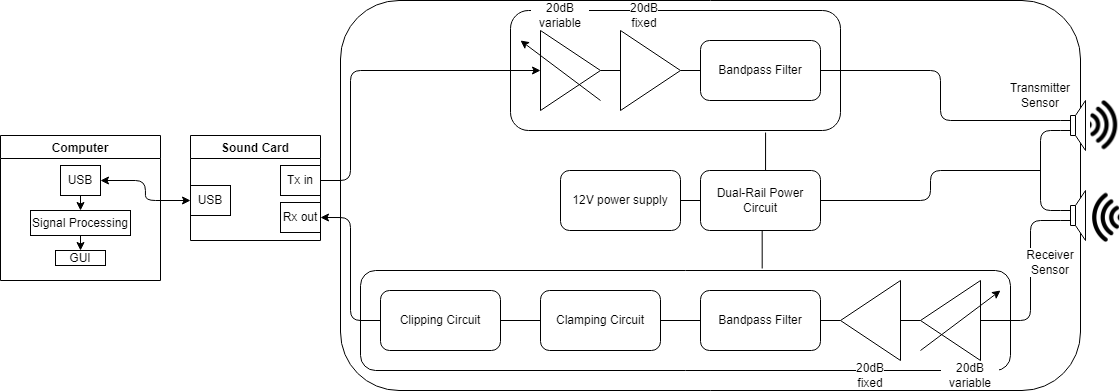
\includegraphics[width=1\columnwidth]{../Images/system_design.png}
    \caption{Overall system operation}
    \label{fig:overall-system-design}
\end{figure}


\section{Transmitter Design}\label{sect:transmitter-design}
The purpose of the transmitter is to receive a 40 kHz \gls{cw} signal from the sound card, amplify it, and filter it through a band-pass filter. The signal is transmitted for a set amount of time. The processed signal is then sent through the ultrasonic barrel transmitter, aimed towards the target of interest. Figure~\ref{fig:transmitter-block} illustrates the operation of the transmitter.

\begin{figure}[htbp]
    \centering
    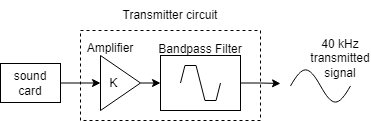
\includegraphics[width=0.6\columnwidth]{../Images/transmitter_block.drawio.png}
    \caption{Block diagram of transmitter operation}
    \label{fig:transmitter-block}
\end{figure}

\subsection{Signal Amplification Requirements}\label{sect:transmitter-signal-amplification}
The system needs to be able to pick up slow-moving vehicles from up to 10 metres away. Hence, an operational amplifier is used to ensure the transmitter has enough power. Due to its low-noise characteristics, an audio operational amplifier was chosen and the amplifier was configured as an adjustable-gain inverting amplifier.

The \gls{gbwp} and slew rate are important parameters to consider when selecting the right operational amplifier. The \gls{gbwp} is calculated using Equation~\ref{eqn:gbwp}, which defines the maximum closed-loop gain that can be achieved by the operational amplifier at the bandwidth of the system.

\begin{equation}
    \text{GBWP} = 10 A_c_l B\:[Hz]
    \label{eqn:gbwp}
\end{equation}

The system is supplied by a 12 V DC source which gives a maximum peak-to-peak voltage of 24 V and input voltage of 3.3 V. The bandwidth of the system is determined by finding the Doppler frequency ranges first. The system should be able to detect vehicles moving at 20 km/h \approx 5.56 m/s.

\begin{center}
\begin{math}
    \lambda = \frac{c}{f} = \frac{343\:m/s}{40\:kHz} = 0.008575\:m \\ \vspace{0.3cm}
    f_D = \frac{2v_r}{\lambda} = \frac{(2)(5.56\:m/s)}{0.008575\:m} = 1296.793\:Hz\\
    \vspace{0.3cm}
    f_L = f_C - f_D = 40\:kHz - 1296.793\:Hz = 38703.207\:Hz\\
    \vspace{0.3cm}
    f_H = f_C + f_D = 40\:kHz + 1296.793\:Hz = 41296.793\:Hz\\
    \vspace{0.3cm}
    \therefore \text{Slew rate} = f_H - 0 = 41296.793\:Hz\\
\end{math}
\end{center}

This bandwidth produces a required \gls{gbwp} of 3 MHz. At this bandwidth, frequencies in the range of 38.7 kHz to 41.3 kHz can be detected by the system.

\begin{center}
    \begin{math}
    \text{GBWP} = (10)\frac{24\:V}{3.3\:V}(41296.793\:Hz) = 3\:MHz
    \end{math}
\end{center}

The slew rate, the rate of change of the output signal, is determined using Equation~\ref{eqn:slew-rate}. 

\begin{equation}
    \text{Slew rate} = 2\pi f V_p_p \times 10^-^6 [V/\mu s]
    \label{eqn:slew-rate}
\end{equation}

With a peak-to-peak voltage of 24 V, a minimum slew rate requirement of 6.23 V/$\mu$s is required.

\begin{center}
    \begin{math}
    \text{Slew rate} = (2\pi)(41296.793\:Hz)(24\:V)(10^{-6}) = 6.23\:V/\mu s
    \end{math}
\end{center}

\subsection{Signal Amplification Implementation}
The operational amplifier used in this design is the MC33079P which is a high quality quad amplifier with a minimum slew rate of 7 V/$\mu$s and \gls{gbwp} of 16 MHz which is sufficient for this design. The amplifier has a dual supply operation of $\pm$5 V to $\pm$18 V, which will be appropriately powered by the 12 V power supply to the system. The specifications of the MC33079P are shown in Table~\ref{tab:mc33079p}.\\

\begin{table}[!htp]
\centering
\caption{\label{tab:mc33079p} MC33079P Technical Specifications}
\vspace{-0.5cm}
\begin{tabular}{|m{14em}|m{3cm}|}
\multicolumn{2}{l}{}\\
\cline{1-2}
Dual supply operation   &   $\pm$5 V to $\pm$18 V\\ \cline{1-2}
Low voltage noise       &   4.5 nV/$\sqrt{Hz}$\\ \cline{1-2}
Low input offset voltage            &   0.15 mV \\ \cline{1-2}
Low T.C. of input offset voltage    &   2 $\mu$V/$\deg$C \\ \cline{1-2}
Total harmonic distortion           &   0.002 \% \\ \cline{1-2}
High Gain Bandwidth Product         &   16 MHz \\ \cline{1-2}
High slew rate          &   7 V/$\mu$s \\ \cline{1-2}
High open loop AC gain  &   800 @ 20 kHz \\ \cline{1-2}
\end{tabular}
\end{table}

The gain of the adjustable inverting amplifier is set using Equation~\ref{eqn:gain} and a 10 k$\Omega$ potentiometer. A maximum gain of 20 dB is achieved using a 10 k$\Omega$ potentiometer for $R_2$ and 1 k$\Omega$ for $R_1$. The configuration of the inverting amplifier is shown in Figure~\ref{fig:amplifier}.

\begin{equation}
    \text{Gain} = - \frac{R_2}{R_1}
    \label{eqn:gain}
\end{equation}

\begin{figure}[htbp]
    \centering
    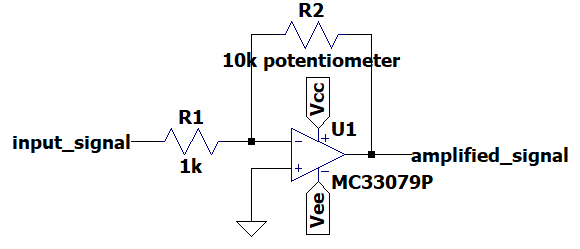
\includegraphics[width=0.6\columnwidth]{../Images/signal_amplification.png}
    \caption{Signal amplification circuit}
    \label{fig:amplifier}
\end{figure}

\subsection{Filter Requirements}
The purpose of the filtering stage is to attenuate frequencies outside the bandwidth range of the transducer. Because the ultrasonic transducer has a bandwidth of approximately 3 - 4 kHz, the filter was designed to attenuate frequencies less than 36 kHz and larger than 44 kHz for a centre frequency of 40 kHz. A two-stage active band-pass filter was chosen to provide an overall gain of 20 dB by having a variable-gain stage that produced 0 dB gain and a fixed-gain stage that produced 20 dB gain. To do this, the low- and high-pass frequencies are determined using Equation~\ref{eqn:low-frequency} and \ref{eqn:high-frequency}.

\begin{subequations}
\begin{equation}
    f_L = \frac{1}{2\pi R_1 C_1}
    \label{eqn:low-frequency}
\end{equation}
\begin{equation}
    f_H = \frac{1}{2\pi R_2 C_2}
    \label{eqn:high-frequency}
\end{equation}
\end{subequations}

The first filter stage was designed with cutoff frequencies of 30 kHz and 50 kHz for $f_L$ and $f_H$, respectively. Using Equation~\ref{eqn:gain}, a gain of 0 dB (linear gain of 1) will require equal resistance values for $R_1$ and $R_2$. Choosing resistor values of 12 k$\Omega$ for $R_1$ and $R_2$, the capacitor values are calculated as $C_1$ = 442 pF and $C_2$ = 265 pF. The second filter stage is required to ensure the response remains centered at 40 kHz with a bandwidth as close to the approximate bandwidth of the transducer as possible. Hence, cutoff frequencies of 36 kHz and 44 kHz were chosen for $f_L$ and  $f_H$, respectively. For a linear gain of 10 (logarithmic gain of 20 dB), resistor values were chosen as $R_1$ = 12 k$\Omega$ and $R_2$ = 120 k$\Omega$. Consequently, the capacitor values are calculated as $C_1$ = 368 pF and $C_2$ = 30  pF.

\subsection{Filter Implementation}
The capacitance values required through calculation are implemented using standard capacitors of 330 pF and 100 pF for $C_1$ and 47 pF and 220 pF capacitors for $C_2$, for the first stage of the filter. The second stage of the filter was implemented with 330 pF and 39 pF capacitors for $C_1$ and a 30 pF capacitor for $C_2$. Figure~\ref{fig:bpf} shows the configuration of the two-stage filter.

\begin{figure}[htbp]
    \centering
    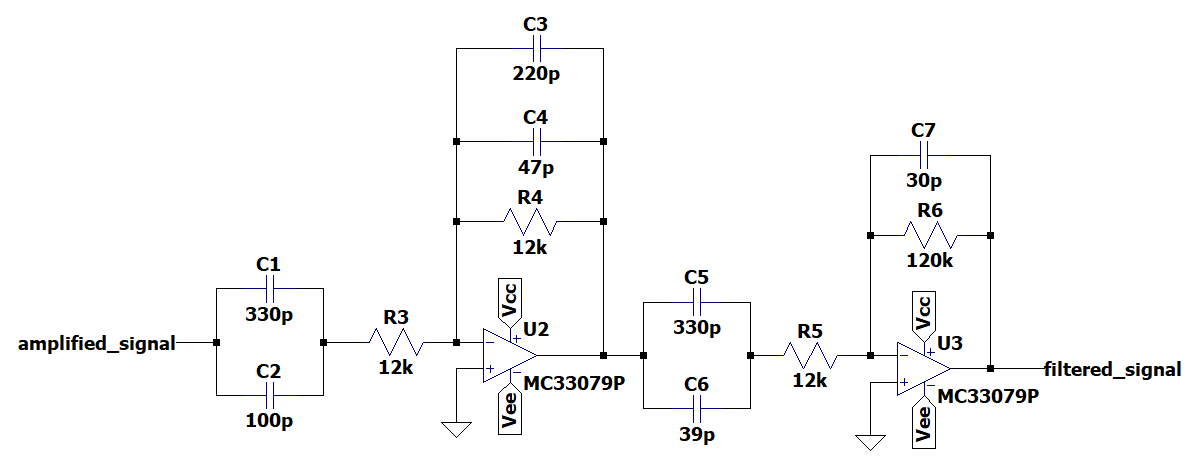
\includegraphics[width=1\columnwidth]{../Images/bandpass_filter.png}
    \caption{Band-pass filter circuit}
    \label{fig:bpf}
\end{figure}

\section{Receiver Design}
Signals in the range of the Doppler frequencies of the system are echoed back towards the receiver. The receiver modifies these echoed signals by amplifying the received signal and filtering it through a band-pass filter. The signal is then clamped to add a \gls{dc} level to the \gls{ac} signal before clipping it to prevent it from exceeding a voltage that could damage the sound card. This process is illustrated in Figure~\ref{fig:receiver-block}.

\begin{figure}[htbp]
    \centering
    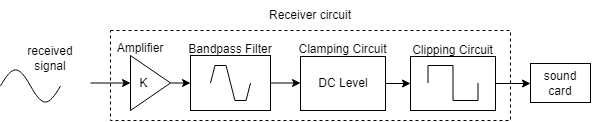
\includegraphics[width=0.85\columnwidth]{../Images/receiver_block.drawio.png}
    \caption{Block diagram of receiver operation}
    \label{fig:receiver-block}
\end{figure}

Because the echoed Doppler frequencies lie in the same range of frequencies as the approximate bandwidth of the ultrasonic transducer, the amplifier and band-pass filter of the receiver is designed to be identical to that of the transmitter as detailed in Section~\ref{sect:transmitter-design}.

\subsection{Clamping Circuit}
The clamping circuit is designed to prevent negative voltages from being sampled by the external sound card (and microcontrollers in the future). This will allow only voltages above 0 V to be sampled. To do this, an inverting op-amp of variable gain was designed using a 10 k$\Omega$ potentiometer and a 12 k$\Omega$ resistor to produce a 3.3 V current. The potentiometer allows the gain to be adjusted to ensure that a voltage of 3.3 V is achieved. A 100 $\mu$F capacitor is used to decouple the output of this op-amp to ground to prevent voltage spikes. A 12 k$\Omega$ resistor and 100 nF capacitor is included between the filter circuit and clamping circuit to prevent the clamping circuit from going into current limiting and the outputs of these two circuits from opposing each other. Figure~\ref{fig:clamping} shows the configuration of this circuit.

\begin{figure}[htbp]
    \centering
    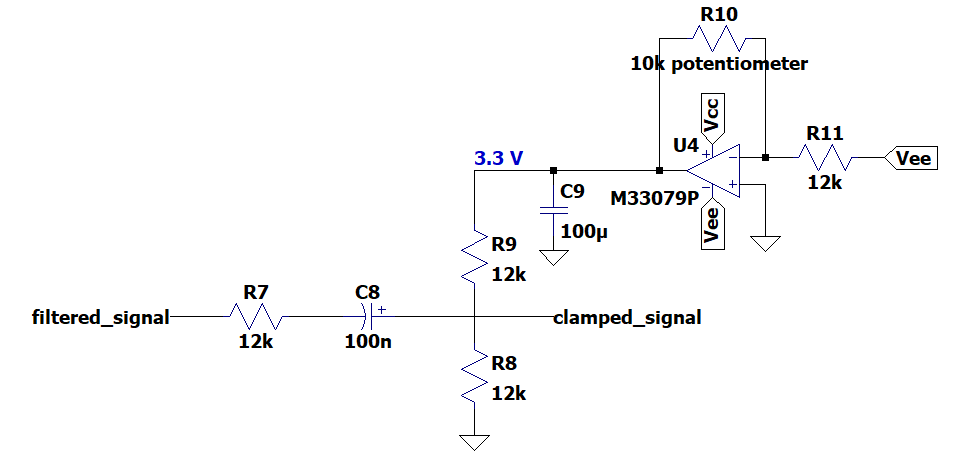
\includegraphics[width=0.8\columnwidth]{../Images/clamping.png}
    \caption{Clamping circuit}
    \label{fig:clamping}
\end{figure}

\subsection{Clipping Circuit}
The maximum output/input voltage of the XONAR U5 sound card is 3.677 V$_{pp}$. This means that voltages above this specification are likely to damage the sound card. To prevent damaging the sound card, the clipping circuit ensures that the input signal to the sound card oscillates in the range of 0 to 3.3 V, saturating voltages outside this range. Two 1N5819 Schottky diodes are connected - one to ground and the other to the 3.3 V signal. Figure~\ref{fig:clipping}.

\begin{figure}[htbp]
    \centering
    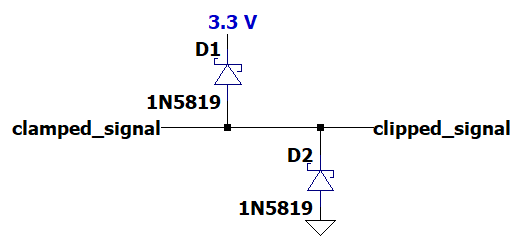
\includegraphics[width=0.6\columnwidth]{../Images/clipping.png}
    \caption{Clipping circuit}
    \label{fig:clipping}
\end{figure}

\section{Power Supply Design}
According to the technical specifications of the MC33079P op-amp in Table~\ref{tab:mc33079p}, the op-amp operates with a dual supply range of $\pm$5 V to $\pm$18 V. To ensure the transmitted and received signals receive enough power, a $\pm$12 V dual rail supply is used to power the op-amps. A power bank that outputs 12 V is used as the power supply. A boost converter is then used to boost the input supply to 24 V before using a rail-splitter circuit to split the voltage into a +12 V and -12 V signal. The MT3608 adjustable voltage regulator was chosen as it allows the voltage supplied to the op-amps to be adjusted between $\pm$5 V and $\pm$12 V, according to the needs of the user. Table~\ref{tab:mt3608} shows the technical specifications of the MT3608. 

\begin{table}[!htp]
\centering
\caption{\label{tab:mt3608} MT3608 Technical Specifications}
\vspace{-0.5cm}
\begin{tabular}{|m{14em}|m{3cm}|}
\multicolumn{2}{l}{}\\
\cline{1-2}
Input voltage               &   2 V to 24 V\\ \cline{1-2}
Fixed switching frequency   &   1.2 MHz\\ \cline{1-2}
Switch current limit        &   4 A\\ \cline{1-2}
Output voltage              &   5 V to 28 V \\ \cline{1-2}
Maximum output current      &   2 A \\ \cline{1-2}
\end{tabular}
\end{table}

Two 12 k$\Omega$ resistors are used in conjunction with an op-amp to split the boosted 24 V supply voltage as illustrated in Figure~\ref{fig:power-supply}. The output of the op-amp is referenced as virtual ground and used as the common ground point for the transmitter and receiver circuitry. The power rails are each decoupled with 100 $\mu$F capacitors to prevent voltage spikes and fluctuations in the signals.

\begin{figure}[htbp]
    \centering
    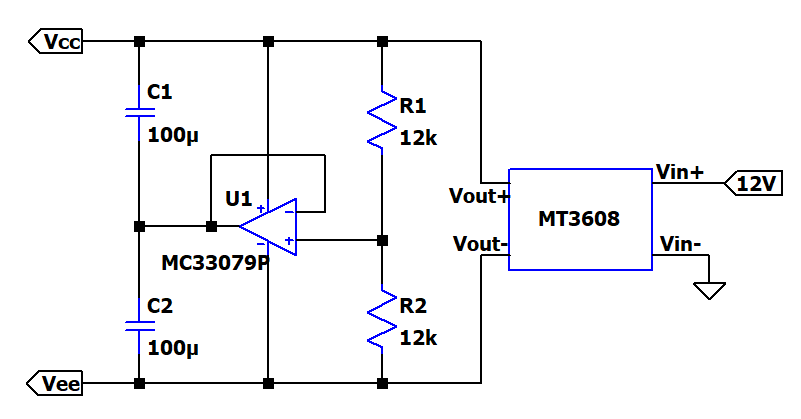
\includegraphics[width=0.45\columnwidth]{../Images/power_supply.png}
    \caption{Power supply circuit}
    \label{fig:power-supply}
\end{figure}

%\href{https://www.electrothinks.com/2021/08/MT3608-2a-dc-to-dc-step-up-power-boost-converter-module.html}{Electrothinks} provides a model circuit diagram of the MT3608 based on its datasheet. This model is used in LTSpice to simulate  realistic results of the power supply design.

\section{Signal Processing Design}
All signal processing was done in \textsc{MATLAB}. A \textsc{MATLAB} script and two functions were written to perform all the processing required. The \textbf{processSignal} function performed the necessary processing on the received signal before the spectrogram could generated. It takes the sampling frequency, transmitting frequency, duration of transmission, and the transmitted and received signal arrays as inputs. The output of this function is a signal that has been adequately processed to ensure an accurate spectrogram can be generated from its data. Figure~\ref{fig:process-signal} shows how the \textbf{processSignal} function works.

\begin{figure}[htbp]
    \centering
    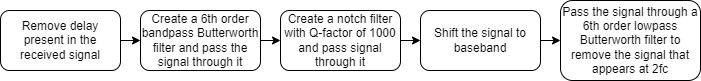
\includegraphics[width=1\columnwidth]{../Images/signal_processing.drawio.png}
    \caption{Operation of processSignal function in \textsc{MATLAB}}
    \label{fig:process-signal}
\end{figure}

The next step in the signal processing design was to create a custom \gls{stft} function that takes the output of the \textbf{processSignal} function and computes the \gls{stft} of this signal. Listing~\ref{lst:customSTFT} shows the code written in \textsc{MATLAB} to create the custom \gls{stft} function. The input to this function is the output signal from the \textbf{processSignal} function, y, the sampling frequency, samples per frame, and overlap factor. The resultant output of this function is a \gls{stft} array, S, and frequency and time vectors f and t, respectively.

\begin{lstlisting}[caption=\textsc{MATLAB} code to create a custom \gls{STFT} function.]
function [S, f, t] = customSTFT(y, Fs, N, OverlapFactor)
    zero_pad = 10*N;
    y = y(:); %convert the signal to a column-vector
    ylength = size(y,1);
    window = hamming(N); %use a window function to get short-time of signal
    overlapSamples = floor(OverlapFactor*N);

    % Get the number of frames to be taken
    hop = N - overlapSamples;
    frames = 1 + floor((ylength-N)/hop);

    % Compute FFT, then apply window to get the STFT
    S = zeros(zero_pad/2+1, frames); % only store positive frequencies in the STFT matrix
    for counter = 0:(frames-1)
        y_window = y(1 + counter*hop : N + counter*hop).*window; %apply window to section of sampled data
        y_fft = fft(y_window, zero_pad);
        y_fft = y_fft(1:zero_pad/2+1)*2;
        S(:,1+counter) = y_fft; %add windowed section to STFT matrix
    end
    
    % Determine frequency and time vectors
    t = (0:hop:(frames-1)*hop)/Fs; 
    f = (0:1:(zero_pad/2))*Fs/zero_pad;
end 
\end{lstlisting}\label{lst:customSTFT}

Finally, a \textbf{customSpectrogram} script is written to compute the instantaneous, average, and maximum speeds from the processed received signal. The operation of this script is displayed in Figure\ref{fig:custom-spectrogram}.

\begin{figure}[htbp]
    \centering
    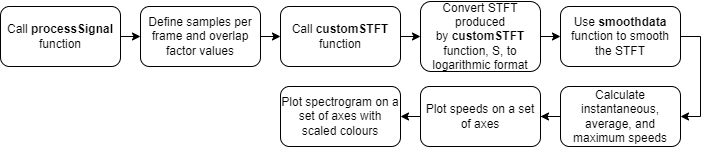
\includegraphics[width=1\columnwidth]{../Images/custom_spectrogram.drawio.png}
    \caption{Operation of customSpectrogram function in \textsc{MATLAB}}
    \label{fig:custom-spectrogram}
\end{figure}

\section{Graphical User Interface}\label{sect:gui}
A simple \gls{gui} is designed in \textsc{MATLAB} using App Designer. This application was designed to be simple and allow the user to easily customise the parameters of the demonstrator. The left panel of the application allows the user to input the frequency of the transmitting signal, the sampling frequency, sampling time, and frame overlap. Brief instructions are provided at the bottom of the panel to ensure the user knows how to use the application. This panel also includes a \textbf{Start logging} button which starts the transmitting and receiving process and processes the received signal. The \textbf{Save data} check box allows the user to save some of the data of the processing to allow them to easily locate the data for post-processing or to retrieve it when needed. This check box saves the cutoff frequency value, sampling frequency value, duration of transmission, and the transmitted and received signal arrays. The right-hand panel displays the instantaneous, average, and maximum speed values on a set of axes with time on the x-axis and speed in km/h on the y-axis. Above this set of axes, the maximum and average speeds detected are displayed in km/h. An important function of the application is that it outputs the spectrogram once the logging process is complete.

\begin{figure}[!htbp]
    \centering
    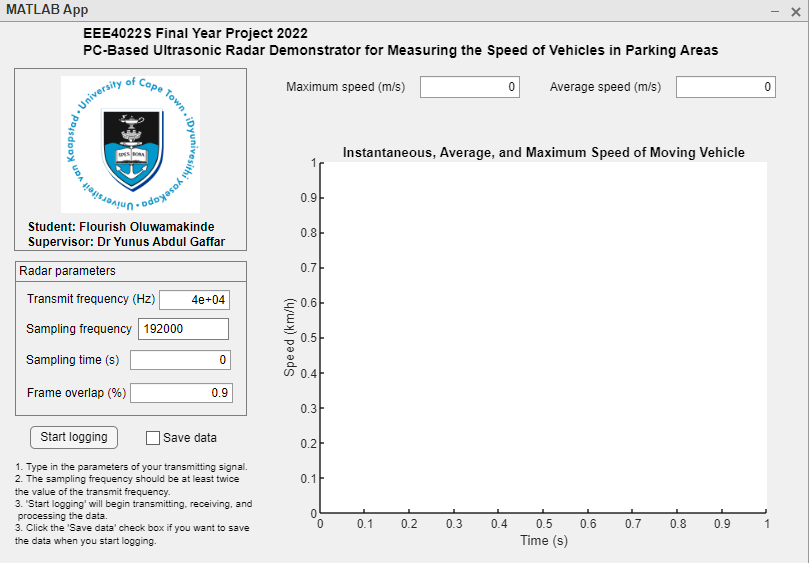
\includegraphics[width=1\columnwidth]{../Images/gui.png}
    \caption{GUI App designed in \textsc{MATLAB}.}
    \label{fig:gui}
\end{figure}

% ----------------------------------------------------
\ifstandalone
\bibliography{../Bibliography/References.bib}
\printnoidxglossary[type=\acronymtype,nonumberlist]
\fi
\end{document}
% ----------------------------------------------------